\JWlone{Evaluation}
\label{sec:evaluation}

What does it mean?


% #  ERROR OF ESTIMATION  ######################################################
\JWltwo{Error of Estimation}
\label{sec:error}

Presentation of measured and estimated work. Plus errors.


% #  COMPARISON TO SIMPLE TIME BASED MODEL  ####################################
\JWltwo{Comparison to a simple time based Model}
\label{sec:time-based}

\begin{figure}
  \centering
    \includegraphics[width=\textwidth]{fig/1cpu-bench-errs.eps}
  \caption{1 CPU error comparison}
  \label{fig:errs-1cpu}
\end{figure}

\begin{figure}
  \centering
    \includegraphics[width=\textwidth]{fig/Ncpu-bench-errs.eps}
  \caption{n CPU error comparison}
  \label{fig:errs-ncpu}
\end{figure}

This chapter features a comparison of the gained energy model to a simple
computing time-(only-)based one. Figures \ref{fig:errs-1cpu} and
\ref{fig:errs-ncpu} illustrate the results. The final energy model worked out in
this thesis (see chapter \ref{sec:final-model}) is listed as \emph{model} in the
figures. The computing time-(only-)based model is built using the performance
event counter \JWctr{CPU\_CLK\_UNHALTED} only and is reffered to in the
figures as \emph{cpu\_time\_model}. Its formula is $5.741J * 10^{-9} *$
\JWctr{CPU\_CLK\_UNHALTED}. It has been fitted using the same training data as
the regular model.

% #  OVERHEAD IMPLEMENTATION  ##################################################
\JWltwo{Overhead of this Implementation}
\label{sec:overhead}

To evaluate the overhead of this implementation three metrics have been used:
Running time, average power usage and unhalted CPU clock cycles. To compare the
results the \emph{473.astar} benchmark of the \emph{Integer Component of SPEC
CPU2006} benchmark suite has been used. Besides a warm-up run every
configuration has been executed ten times. The performance events have been
added consecutively in the order they are listed in appendix
\ref{appendix:chosen-events}. Before measuring the costs of adding a counter,
the system has been benchmarked without even setting up \JWTlibpfm{} (see
chapter \ref{sec:standard-software}). In the plots these configurations are
listed as \emph{0} performance events measured. Because the unhalted CPU clock
cycles are measured using the PMU (chapter {\ref{sec:pmu}) and \JWTlibpfm{}
there is obviously no benchmark without even setting up \JWTlibpfm{}.

\begin{figure}
  \centering
    \includegraphics[width=\textwidth]{fig/ctr-csts-cycles.eps}
  \caption{Counter Costs Cycles}
  \label{fig:ctr-costs-cycles}
\end{figure}

\begin{figure}
  \centering
    \includegraphics[width=\textwidth]{fig/ctr-csts-time.eps}
  \caption{Counter Costs Time}
  \label{fig:ctr-costs-time}
\end{figure}

\begin{figure}
  \centering
    \includegraphics[width=\textwidth]{fig/ctr-csts-power.eps}
  \caption{Counter Costs Power}
  \label{fig:ctr-costs-power}
\end{figure}

As one can see in figures \ref{fig:ctr-costs-cycles} and
\ref{fig:ctr-costs-time}, the number of counted performance events or using the
PMU (see chapter \ref{sec:pmu}) does not seem to correlate to the clock
cylces to CPU works or the time a process needs to complete. The
Pearson product-moment correlation coefficients\cite{wiki:PCC} are $-0.18$ with
repect to the running time and $-0.12$ to the clock cycles. Considering the
average electrical power there's some correlation (PCC: $0.72$, figure
\ref{fig:ctr-costs-power}), but the absolute value ($<$ \SI{0.3}{\watt}) is
negligible.

The result is that this implementation does not harm the system's performance or
its energy usage.


% #  VARIATION BETWEEN RUNS  ###################################################
\JWltwo{Variation of Results between Runs}
\label{sec:variation}

Are there variations of the results between the runs?
